\chapter{Results}
\begin{center}
\vspace{-6ex}
\textit{"Cut to the chase"}
\vspace{6ex}
\end{center}


\section{Image segmentation}

\subsection{Data set 1}

\begin{figure}[H]
    \centering
    \captionsetup[subfigure]{justification=centering}
    \begin{subfigure}[b]{0.3\textwidth}
        \centering
        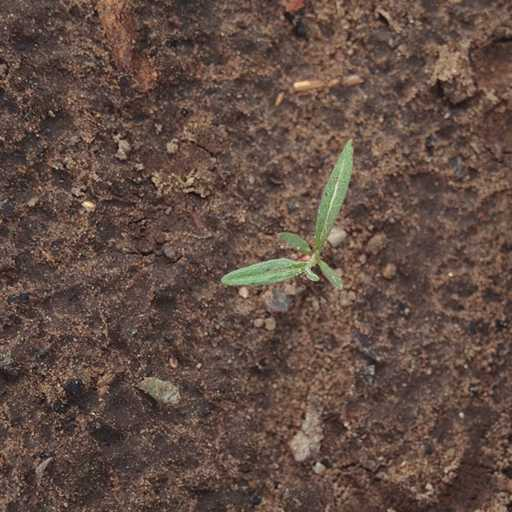
\includegraphics[width=\textwidth]{./figure/result/segmentation/imgORIGINAL.png}
		\caption{}
		\label{fig:seg_a}
    \end{subfigure}
    \begin{subfigure}[b]{0.3\textwidth}
        \centering
        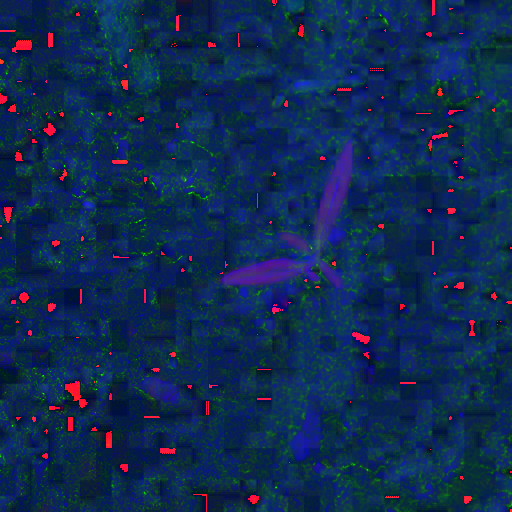
\includegraphics[width=\textwidth]{./figure/result/segmentation/imgHSI.png}
        \caption{}
		\label{fig:seg_b}
    \end{subfigure}
    \begin{subfigure}[b]{0.3\textwidth}
        \centering
        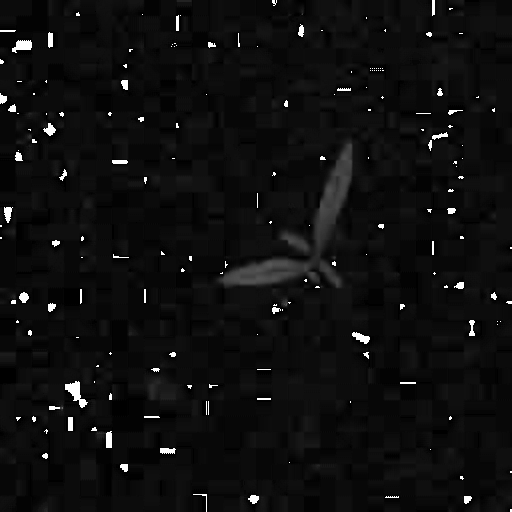
\includegraphics[width=\textwidth]{./figure/result/segmentation/imgHSI1.png}
		\caption{}
		\label{fig:seg_c}
    \end{subfigure}
    \begin{subfigure}[b]{0.3\textwidth}
        \centering
        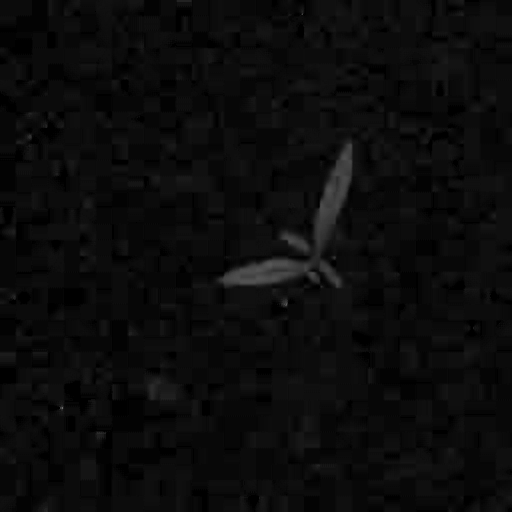
\includegraphics[width=\textwidth]{./figure/result/segmentation/imgHSIClean.png}
		\caption{}
		\label{fig:seg_d}
    \end{subfigure}
    \begin{subfigure}[b]{0.3\textwidth}
        \centering
        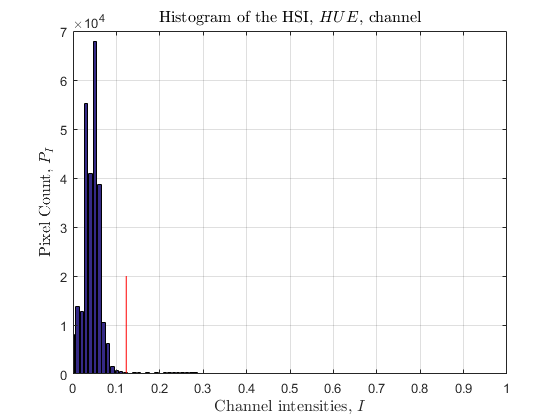
\includegraphics[width=\textwidth]{./figure/result/segmentation/imgCLIPPING.png}
		\caption{}
		\label{fig:seg_e}
    \end{subfigure}
    \begin{subfigure}[b]{0.3\textwidth}
        \centering
        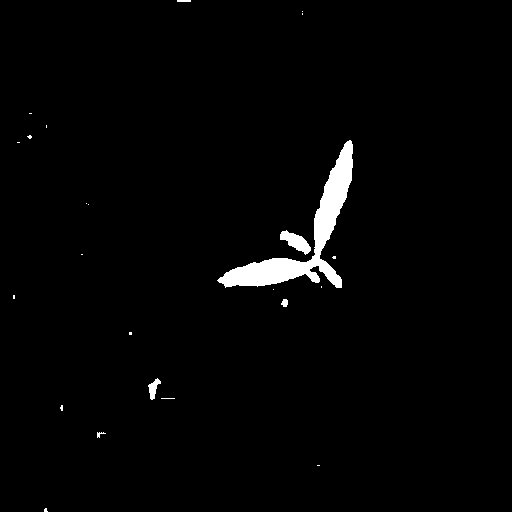
\includegraphics[width=\textwidth]{./figure/result/segmentation/imgHSIThreshold.png}
		\caption{}
		\label{fig:seg_f}
    \end{subfigure}
    \begin{subfigure}[b]{0.3\textwidth}
        \centering
        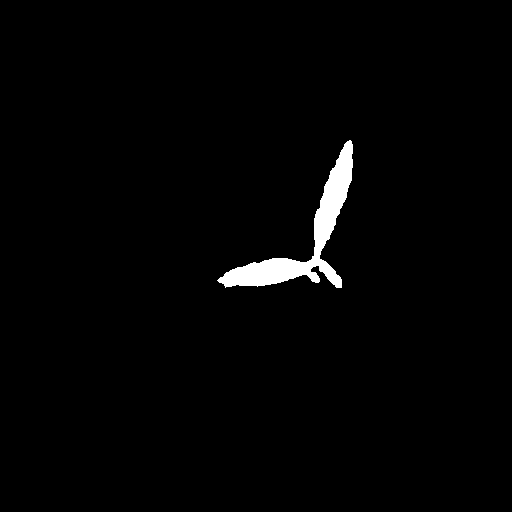
\includegraphics[width=\textwidth]{./figure/result/segmentation/imgHSIThresholdClean.png}
		\caption{}
		\label{fig:seg_g}
    \end{subfigure}
    \begin{subfigure}[b]{0.3\textwidth}
        \centering
        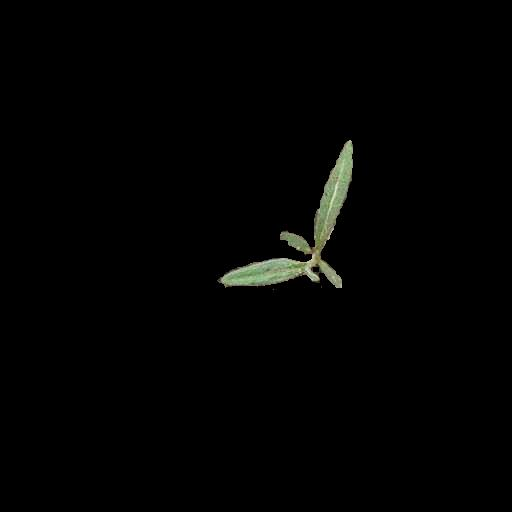
\includegraphics[width=\textwidth]{./figure/result/segmentation/imgSEG.png}
		\caption{}
		\label{fig:seg_h}
    \end{subfigure}
    \caption{The segmentation process as follows: \textit{(a):} The original image is loaded and prepared for processing. \textit{(b):} The image converted to HSI but still represented in RGB colours. \textit{(c):} For the segmentation to work properly the image needs to be represented in one channel that represents the two segments well, and this is what the Hue channel in HSI representation does. \textit{(d):} The Hue channel clean up. \textit{(e):} The optimal threshold between the two segments is represented by the red line  \textit{(f):} Binarization of the HSI image using clipping. \textit{(g):} Clean up the binary image by removing small objects. \textit{(h):} Final segmented image.  }
    \label{fig:1}
\end{figure}

\subsection{Data set 2}

\begin{figure}[H]
    \centering
    \captionsetup[subfigure]{justification=centering}
    \begin{subfigure}[b]{0.47\textwidth}
        \centering
        \includegraphics[width=\textwidth]{./figure/result/segmentation_my/imgOrig.jpg}
		\caption{}
		\label{fig:seg_a}
    \end{subfigure}
    \begin{subfigure}[b]{0.47\textwidth}
        \centering
        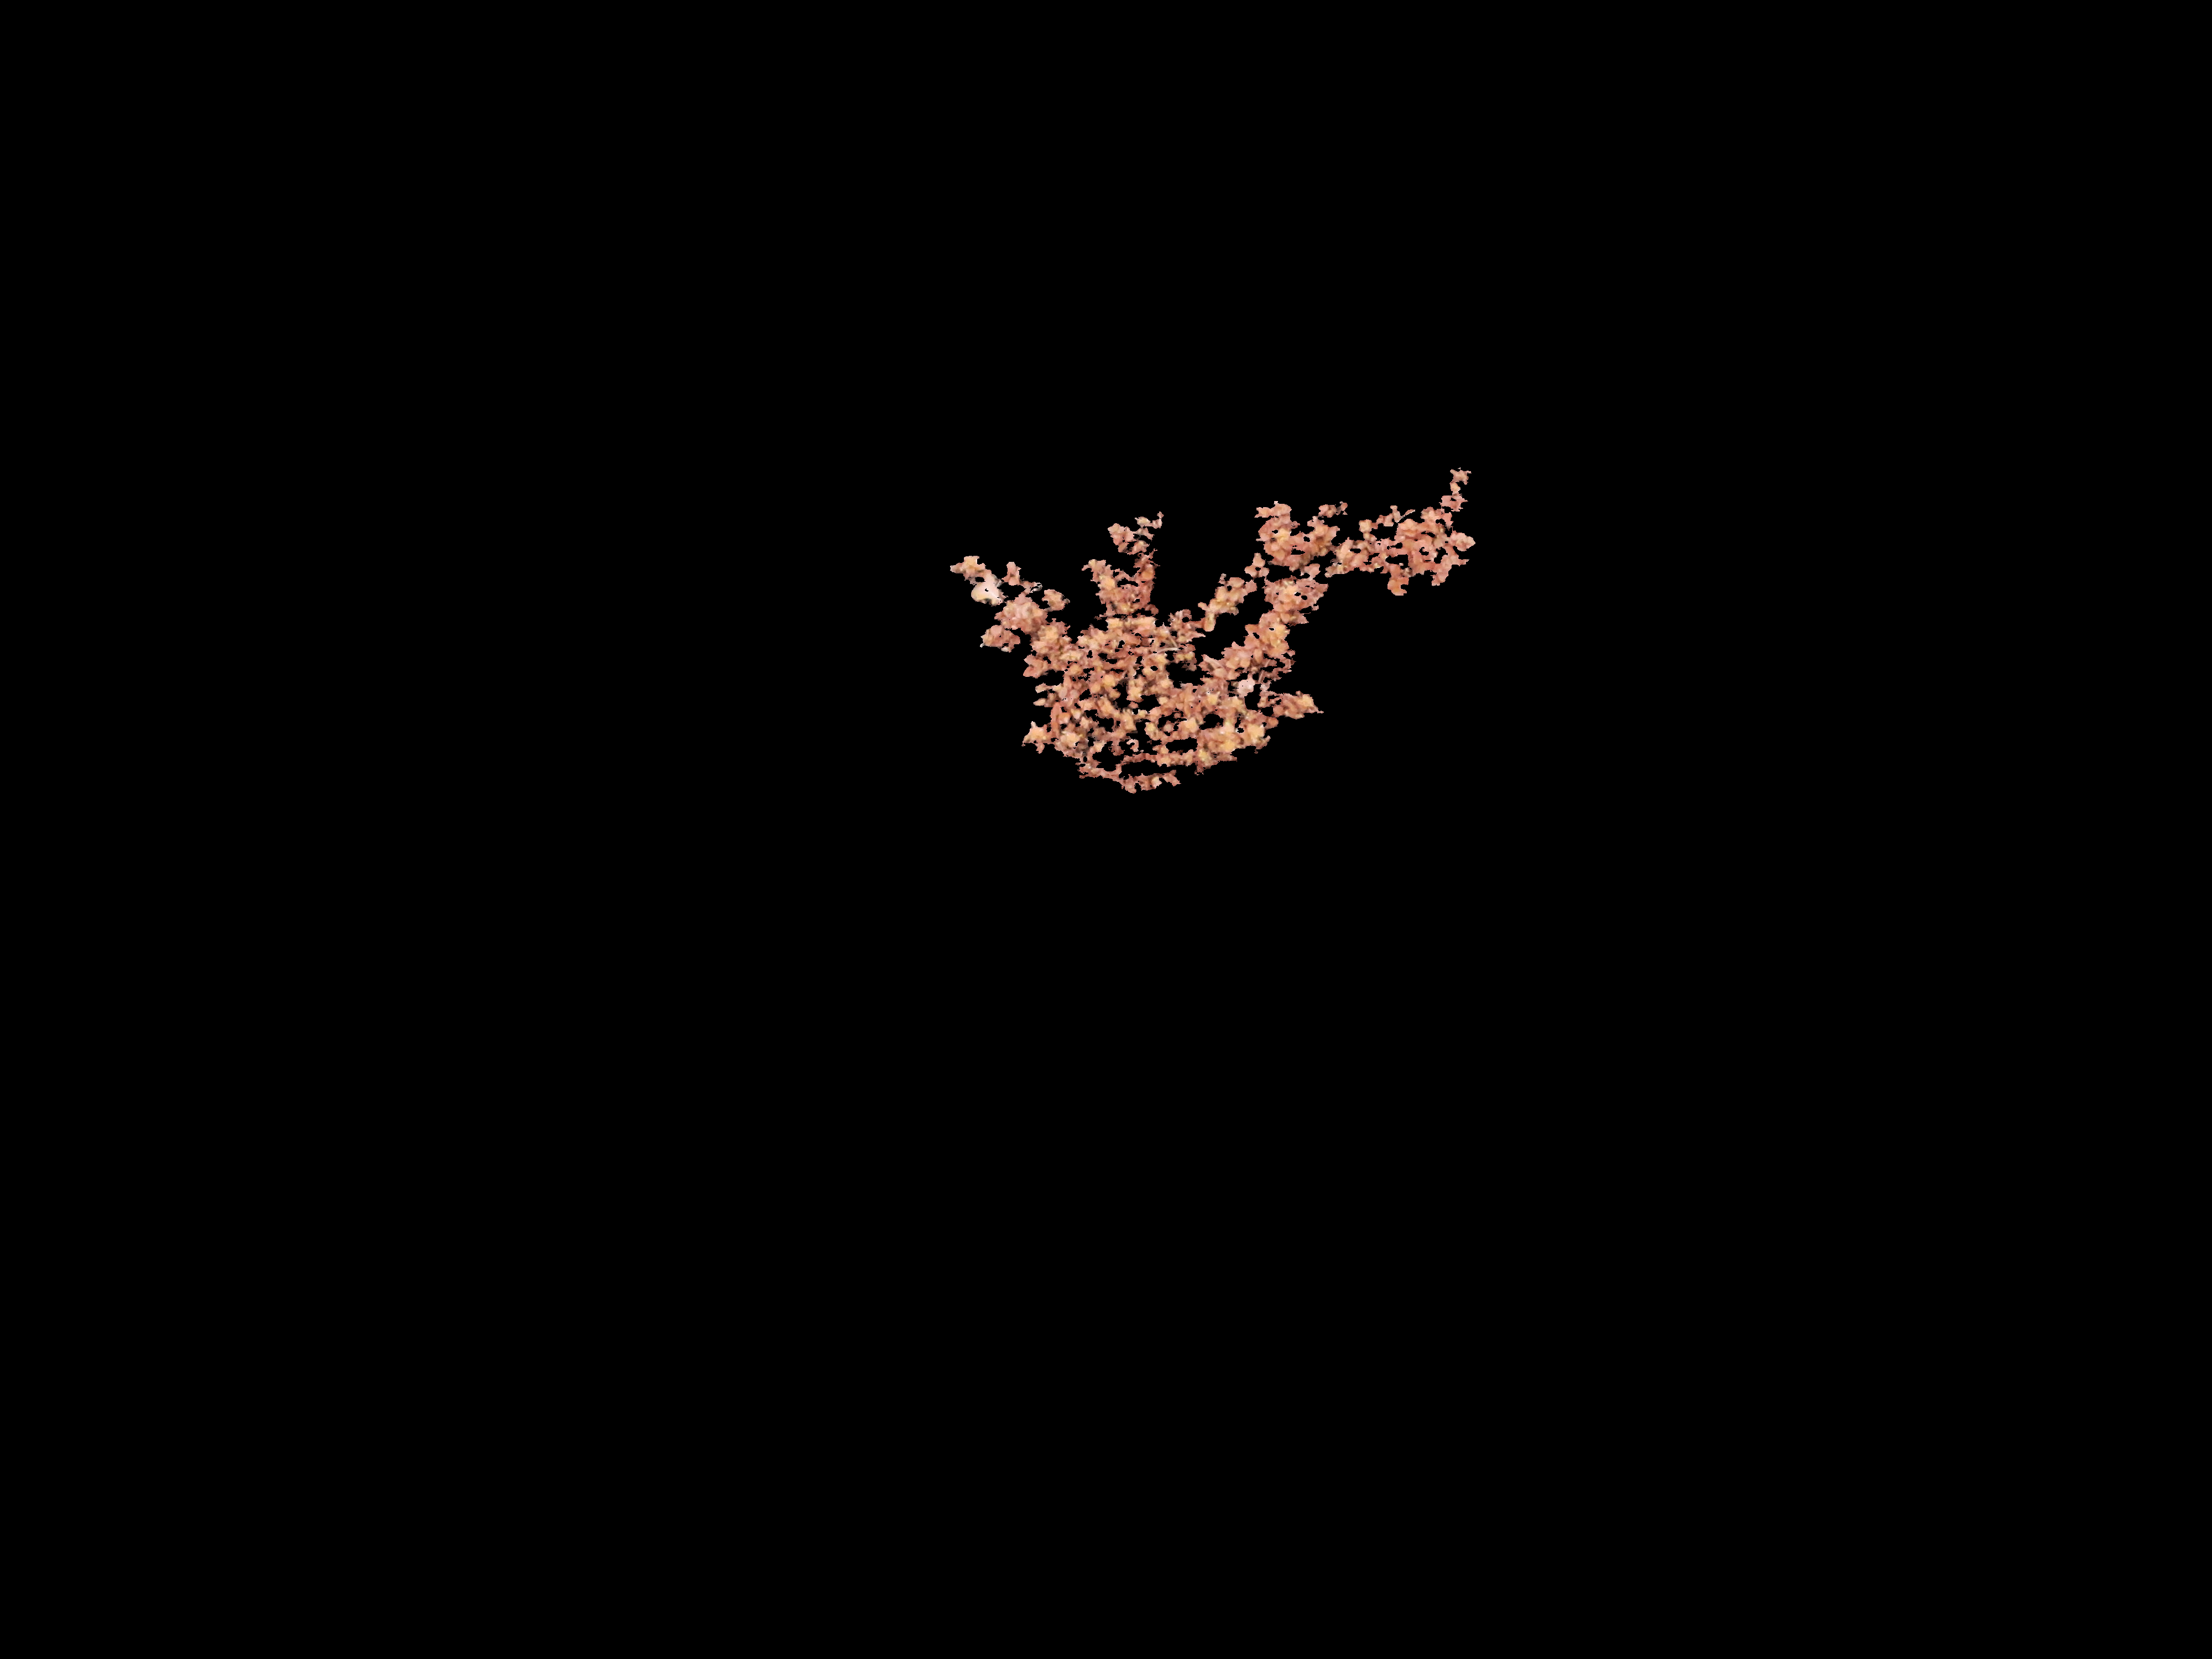
\includegraphics[width=\textwidth]{./figure/result/segmentation_my/imgSeg.png}
        \caption{}
		\label{fig:seg_b}
    \end{subfigure}
    \caption{Directly applying the same segmentation algorithm on non-perfect noise data does not really give satisfying results.}
    \label{fig:result_segmentation_2}
\end{figure}

Using the same algorithm on the data received on a field without alterations, and also quite late in the development does not give good result as can be seen in figure \ref{fig:result_segmentation_2}. This is due several reason, first we can see that there are more than one interesting plant in the picture, and from the results we see that only a part of a plant is given. This is where the convolutional neural networks come in for the first time, using a convolutional neural network one can train the networks to segment the image into several important parts. Using this network to classify segments of an image could be done as prework and then the normal classification using a normal feed forward network or just the quadratic classifier, but why stop here when we have already integrated a CNN, why not use it in series with another CNN to only train one big network instead of using several different parts of the classification.


\section{Method}
\section{}
Återger resultat från observationer och datorstödda
analyser/mätningar. Vanligtvis återges resultat i form av
figurer, tabeller, grafer, eller fotografier men det är avgörande
att även förse dessa med tillräckliga kommentarer för att belysa
resultatets värde och eventuella avvikelser eller oväntade
resultat. Givetvis ska resultatavsnittet också bestå av text som
binder samman illustrationerna.
Beroende på experiment eller metod bör skribenter ange och
berättiga beräkningar och formler som ligger till grund för
tolkningen av resultat och datorstödd analys. I vissa fall måste
även primärdata anges för att resultat ska bli meningsfulla och
kunna diskuteras. Med primärdata avses obehandlade mätdata.
Notera att detta inte är tillämpligt i alla enskilda fall. Fråga din
ämneshandledare.





\section{Results from quadratic discrimination}

\begin{table}[H]
\centering
\caption{Feature names along with their corresponding feature number during feature selection phase.}
\label{tab:featNameNum}
\begin{tabular}{|l|l|l|l|l|l|}
\hline
\textbf{\begin{tabular}[c]{@{}l@{}}Feature \\ Number\end{tabular}} & \multicolumn{1}{c|}{1}                                   & \multicolumn{1}{c|}{2}                                   & \multicolumn{1}{c|}{3}                                   & \multicolumn{1}{c|}{4}                                      & \multicolumn{1}{c|}{5}                              \\ \hline
\textbf{\begin{tabular}[c]{@{}l@{}}Feature \\ Name\end{tabular}}   & Form factor                                                     & Elognatedness                                                     & Convexities                                                     & Solidities                                                       & \begin{tabular}[c]{@{}l@{}}Mean \\ Red\end{tabular} \\ \hline
\textbf{\begin{tabular}[c]{@{}l@{}}Feature \\ Number\end{tabular}} & \multicolumn{1}{c|}{6}                                   & \multicolumn{1}{c|}{7}                                   & \multicolumn{1}{c|}{8}                                   & \multicolumn{1}{c|}{9}                                      & \multicolumn{1}{c|}{10}                             \\ \hline
\textbf{\begin{tabular}[c]{@{}l@{}}Feature \\ Name\end{tabular}}   & \begin{tabular}[c]{@{}l@{}}Mean \\ green\end{tabular}    & \begin{tabular}[c]{@{}l@{}}Mean \\ blue\end{tabular}      & \begin{tabular}[c]{@{}l@{}}Standard \\ Deviation \\ Red\end{tabular}       & \begin{tabular}[c]{@{}l@{}}Standard \\ Deviation \\ Red\end{tabular}        & \begin{tabular}[c]{@{}l@{}}Std \\ blue\end{tabular} \\ \hline
\textbf{\begin{tabular}[c]{@{}l@{}}Feature \\ Number\end{tabular}} & \multicolumn{1}{c|}{11}                                  & \multicolumn{1}{c|}{12}                                  & \multicolumn{1}{c|}{13}                                  & \multicolumn{1}{c|}{14}                                     & \multicolumn{1}{c|}{}                               \\ \hline
\textbf{\begin{tabular}[c]{@{}l@{}}Feature \\ Name\end{tabular}}   & \begin{tabular}[c]{@{}l@{}}Area\\  Moment 1\end{tabular} & \begin{tabular}[c]{@{}l@{}}Area \\ Moment 2\end{tabular} & \begin{tabular}[c]{@{}l@{}}Area\\  Moment 3\end{tabular} & \begin{tabular}[c]{@{}l@{}}Perimeter \\ Moment\end{tabular} &                                                     \\ \hline
\end{tabular}
\end{table}

\begin{figure}[H]
\centering
%%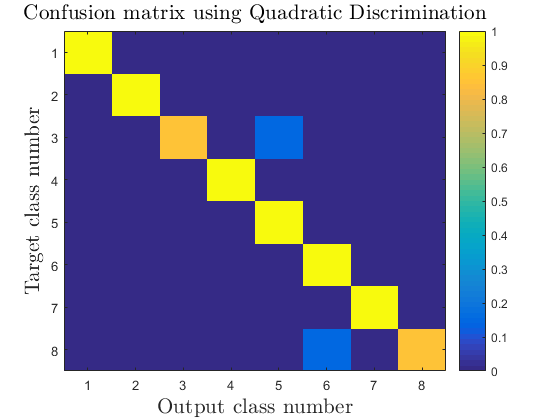
\includegraphics[width=0.5\textwidth]{./figure/result/Quadratic/confusion.png}
\caption{\label{fig:resut_quadratic_confusion}}
\end{figure}

\begin{figure}[H]
    \centering
    \begin{subfigure}[b]{0.47\textwidth}
        \centering
        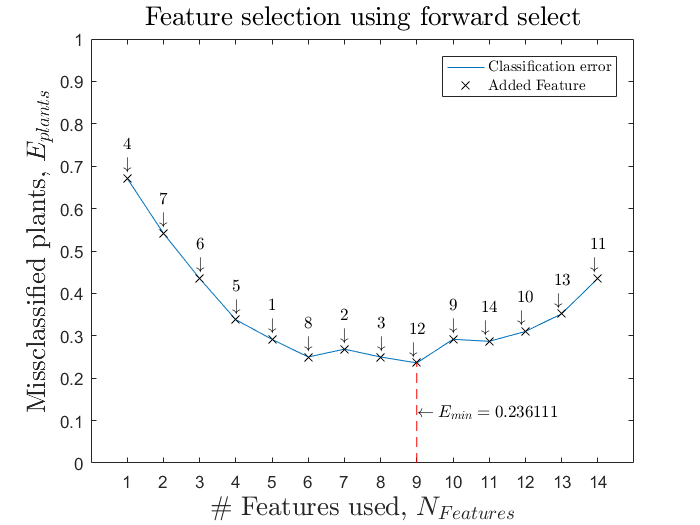
\includegraphics[width=\textwidth]{./figure/result/Quadratic/forward.png}
    \end{subfigure}
    \begin{subfigure}[b]{0.47\textwidth}
        \centering
        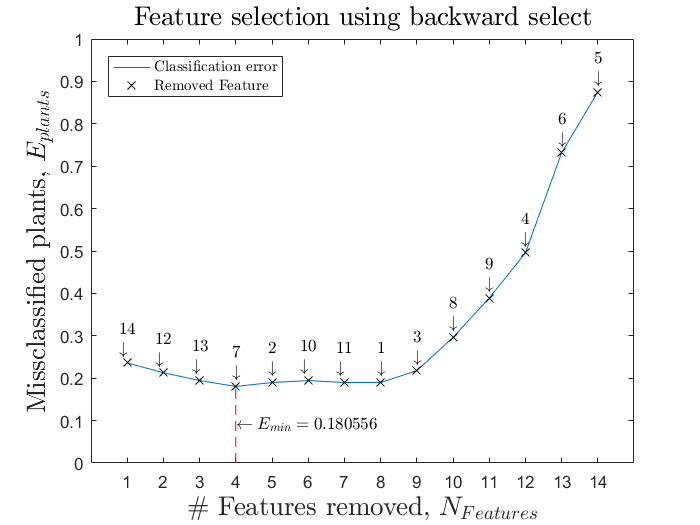
\includegraphics[width=\textwidth]{./figure/result/Quadratic/backward.png}
    \end{subfigure}
    \caption{\label{fig:backforSelection} Using either forward or backward selection for the best feature combination yields different results. E.g. Feature number 7 (mean blue) is the second feature to be added in the forward selection algorithm and is the last to be removed in the backward selection. The corresponding features can be found in Table~\ref{tab:featNameNum}.}
\end{figure}

\begin{figure}[H]
\centering
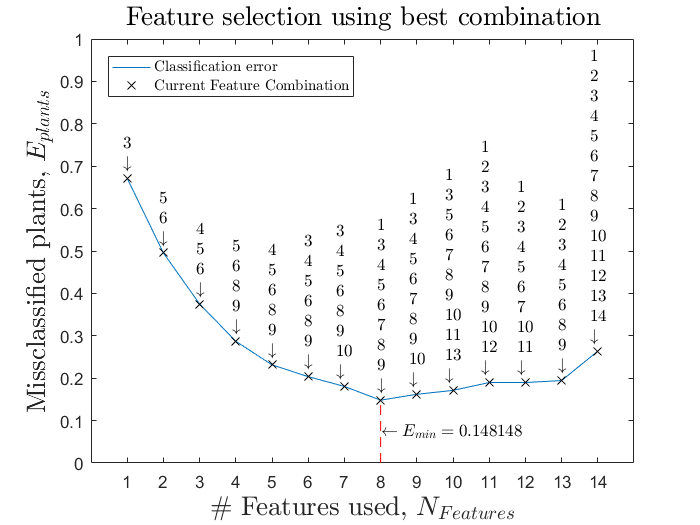
\includegraphics[width=0.47\textwidth]{./figure/result/Quadratic/combination.png}
\caption{\label{fig:combSelection} With immense computer power the best $n$ combinations can be brute forced. This ensures to get the best available combination using $n$ features as all combinations are compared to each other.  }
\end{figure}

As we can see in Figure~\ref{fig:backforSelection}, many of the defined features are present when selecting the best combinations of features using both the backward and forward selection algorithm. In both cases, the class of features which are neglected the most are the moment invariant features. During these algorithms $K-$crossvalidation was used with $K=3$, i.e. the different plants was randomly divided into 9 different group with 3 plants in each. This grouping is different in each run and might thus yield different results for different runs. To make this more consistent, the grouping could be done using increasing the dart wheel as in Figure~\ref{fig:dartWheel} indexing instead of the random distribution in Figure~\ref{fig:randomWheel}.

With much patients the absolute best combination was found by combining the best $n$ features together. This can be seen in Figure~\ref{fig:combSelection}. The result from using this algorithm will only be used in a best case scenario when comparing to other methods later as this algorithm is very slow compared to the other. The feature selection process usually takes place before the classification is done, thought, if one would find a new feature that might give more information this whole process would need to be made again and thus a fast algorithm is preferred.




\section{Results from neural networks}

\section{Unsupervised problem}
